The second paper utilised the age-dependent liability threshold (ADuLT) model, which is the model underlying LT-FH++. The purpose of the project was to examine the performance of the ADuLT outcome with established time-to-event GWAS methods that are based on the Cox proportional hazards model. It is two fundamentally different ways to approach time-to-event analysis in a GWAS setting. The adoption of Cox PH models in a GWAS setting has been limited, which has also been evident in the relative lack of method developments for Cox PH models compared to linear regression models. One of the main limitations for Cox PH is the computational cost of such a model, which has limited GWASs to less than $ 20,000 $ individuals with these models. Recently, a method called SPACox \cite{bi2020fast} has been proposed that allows for far better scaling, and allowing for analysis of UKBB sized biobanks. 


\subsubsection{Simulation results}

Similar to the first paper, we assessed the models in simulations first. In this project, we simulated the genotypes and assigned phenotypes with two generative models. The first model was the liability threshold model and the second model was the proportional hazards model. Notably, one would expect a method based on the liability threshold model to perform the best under this model, and subpar under other generative models. The simulation results shown in Figure \ref{fig:adult_simulations} show the power for $ 10 $ replications under two different generative models and for different population prevalences. For Figure \ref{fig:adult_simulations}A, we observe the expected ranking between methods, since the ADuLT or case-control status methods perform slightly better than the Cox PH model and vice versa. Notably, there is no case ascertainment in those simulations. In results shown in Figure \ref{fig:adult_simulations}B are with case ascertainment and we observe a large shift in power between methods and generative models. In short, the simulation results with case ascertainment show that the Cox PH based method has a far lower power than the LTM based methods under \textit{both} generative models. Even after performing inverse probability weighing Cox PH on a select subset of null SNPs, we observed the same result. This indicates that the Cox PH models with the current implementation suffers from a significant power loss when case ascertainment is present in a GWAS setting.
\begin{wrapfigure}{L}{10cm}
	\label{fig:adult_simulations}
	\caption{ADuLT simulations}
	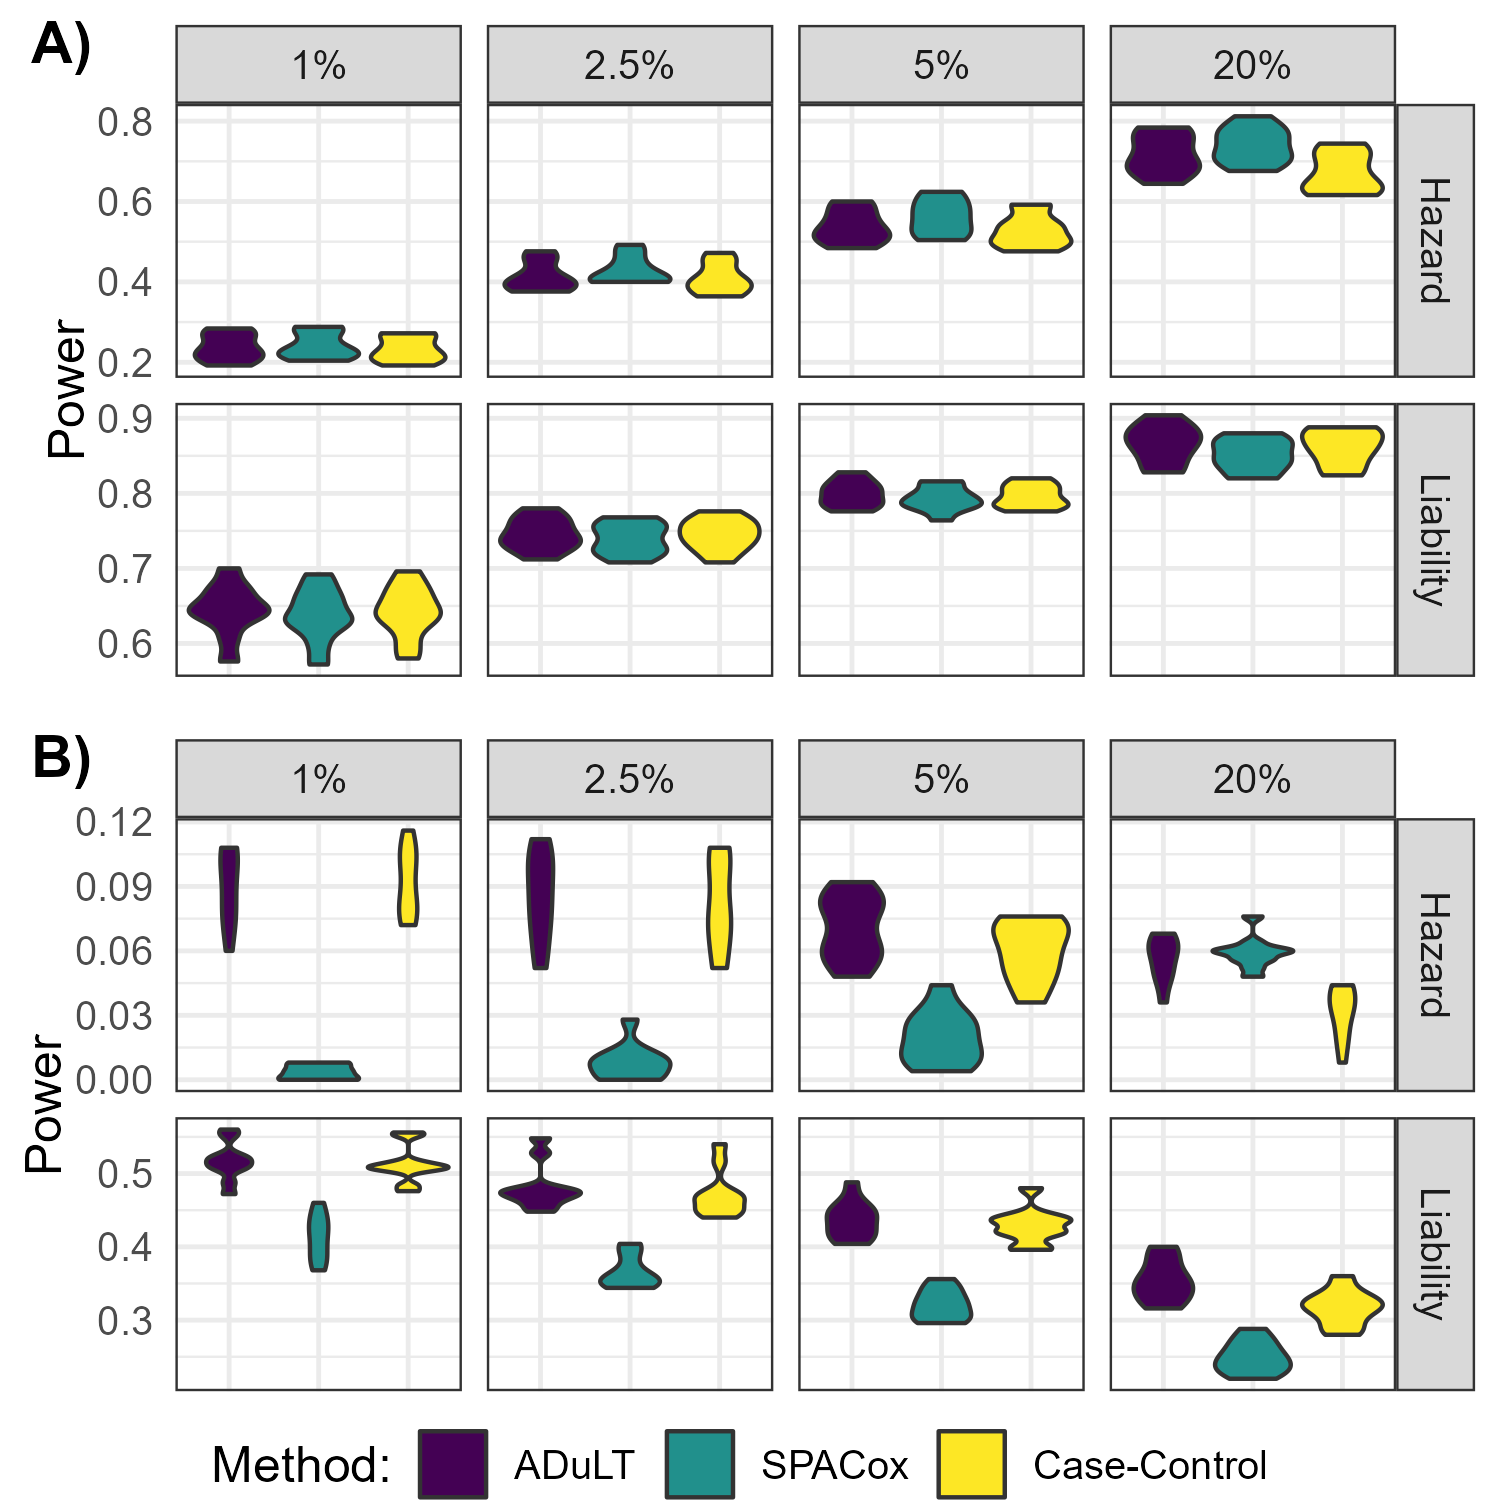
\includegraphics[width=10cm]{results/adult_combined_C250_power}
\end{wrapfigure}


\subsubsection{Real-world analysis}
Next, we applied the same analysis to real-world data to assess whether we observed the same with case ascertainment present in the data. iPSYCH is particularly useful for this, as all cases in a given time period have been sampled and sequenced, meaning the iPSYCH data has the highest possible case ascertainment in real-world data. 

\begin{wrapfigure}{L}{9cm}
	\label{fig:adult_ADHD}
	\caption{ADuLT manhattan plot}
	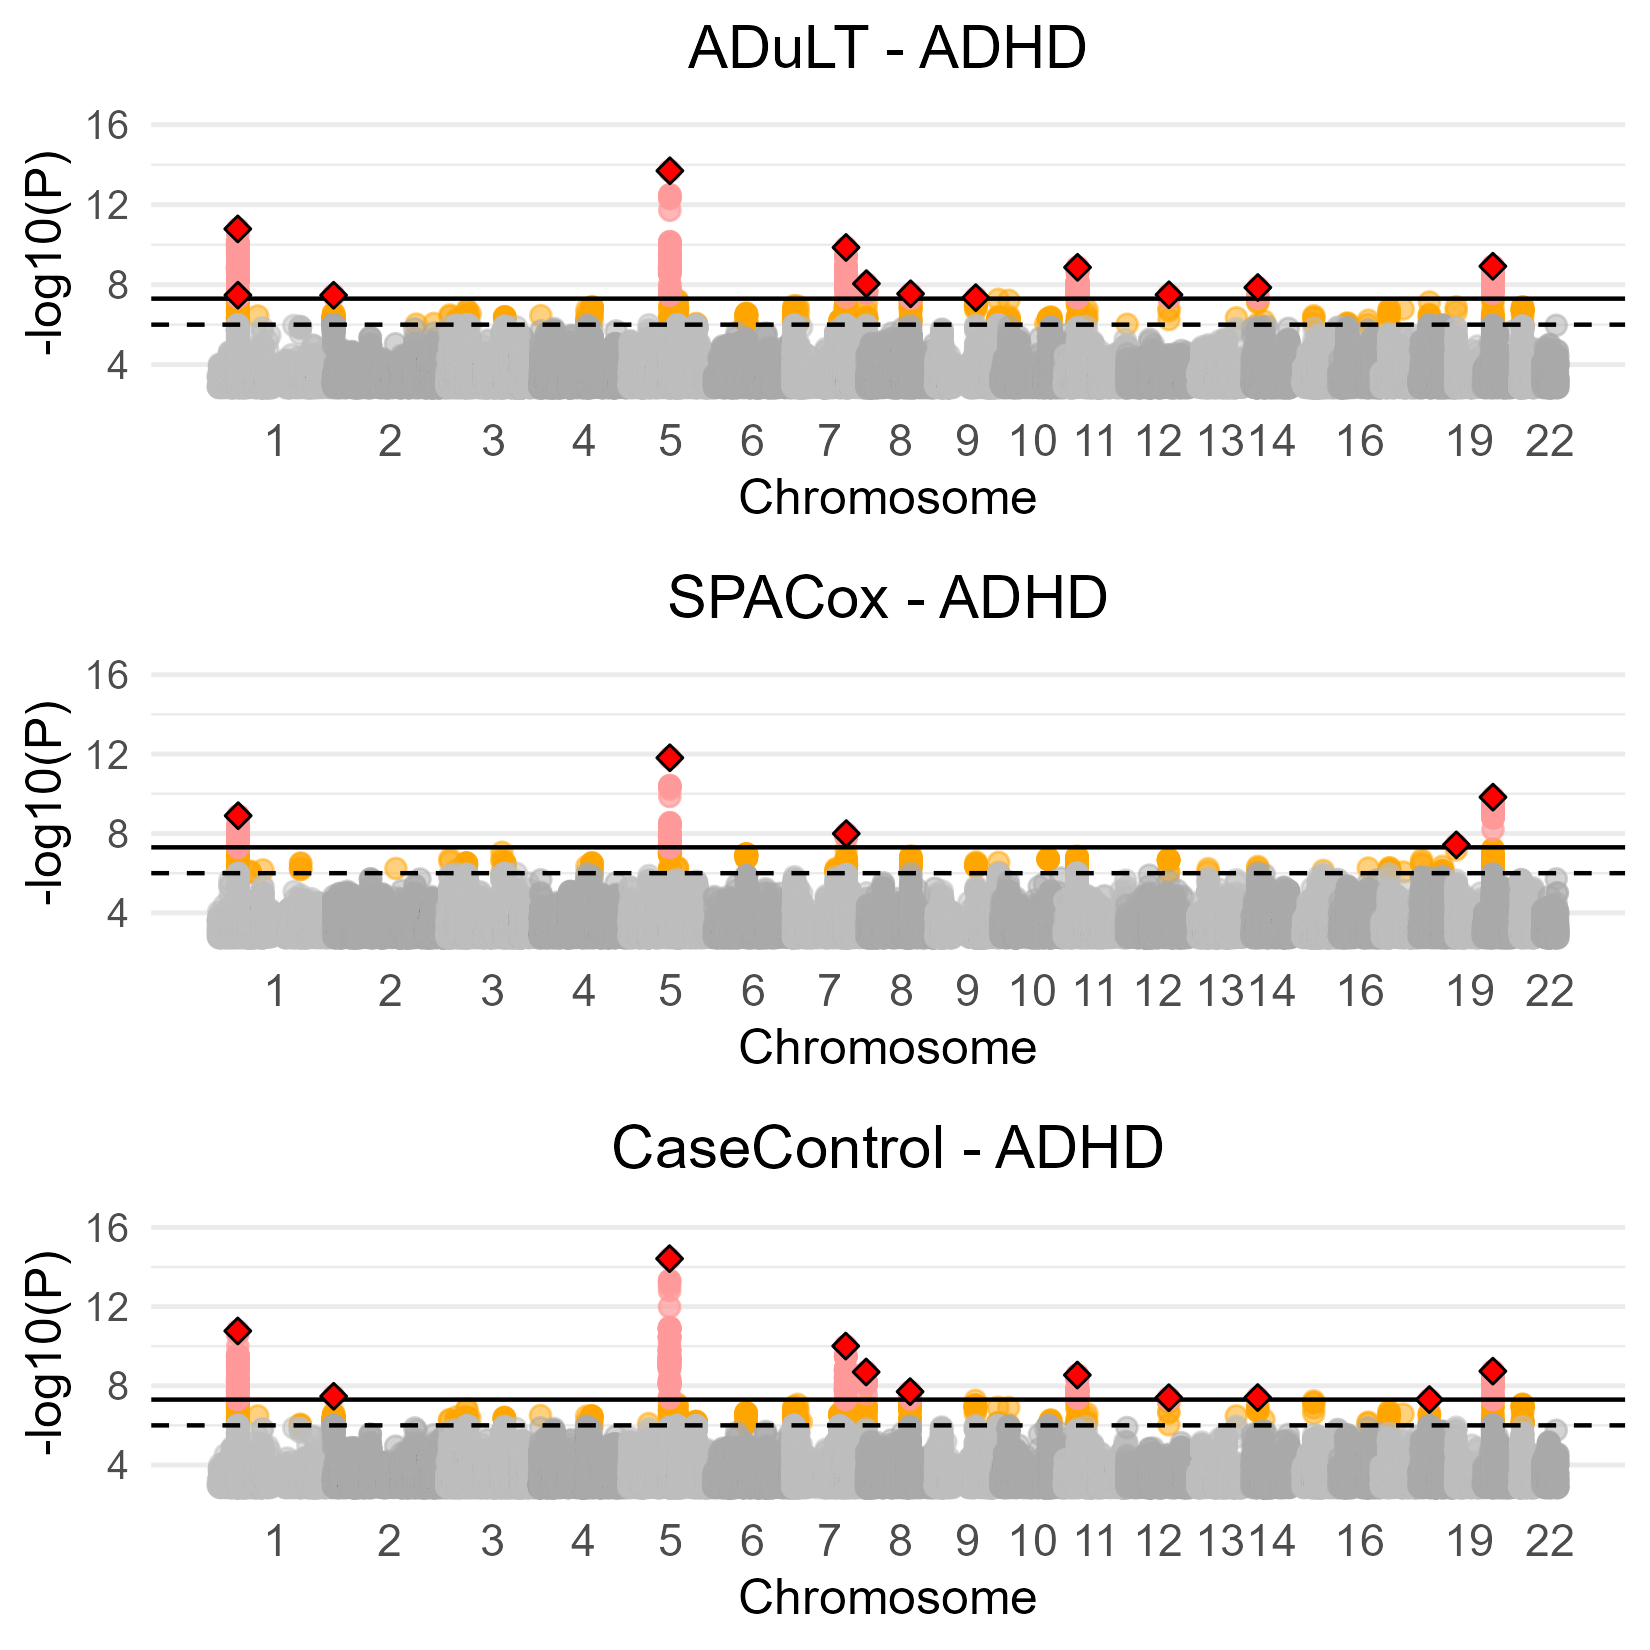
\includegraphics[width=9cm]{results/adult_manhattanPlot_ADHD}
\end{wrapfigure}
We found that ADuLT and case-control status performed better than the Cox PH model by a rather significant margin. In no circumstances did the Cox PH model outperform a LTM based method, showing that the currently implementation of Cox PH model do not perform as well as simpler models such as linear regression, which are also far more computationally efficient.

